\section{Performance of MUMPS in case of Small Systems of Equations}
\label{subseq:small-matrices}

During testing described in sections BRA, BRA and BRA, we observed that execution time grew with increase of processing elements in case of relatively small systems of equations such as \textit{cube-5} and \textit{pwr-3d}. Figure \ref{fig:mumps-small-matrices-total-time} shows parallel performance of MUMPS-OpenBLAS configuration with using flat-MPI mode for the smallest matrices in GRS matrix set.


\figpointer{\ref{fig:mumps-small-matrices-total-time}}
\begin{figure}[htpb]
\centering
	\begin{tabular}{cc}
		\subfloat[pwr-3d]{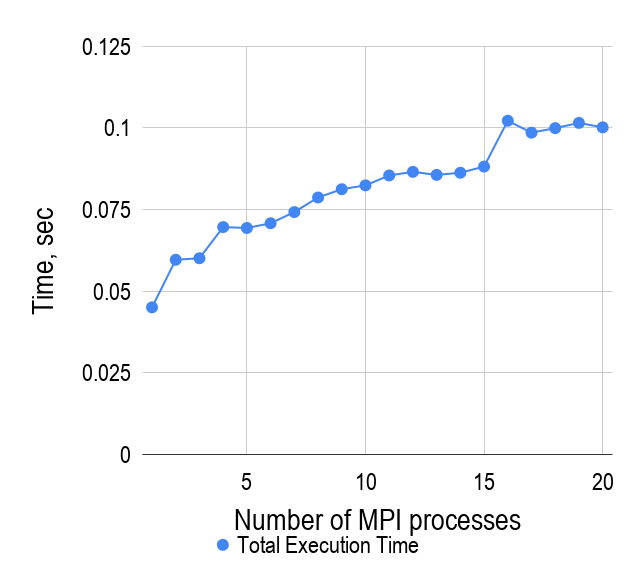
\includegraphics[width=0.475\textwidth]{figures/chapter-2/small-matrices/total-time-pwr-3d.png}} &
		\subfloat[cube-5]{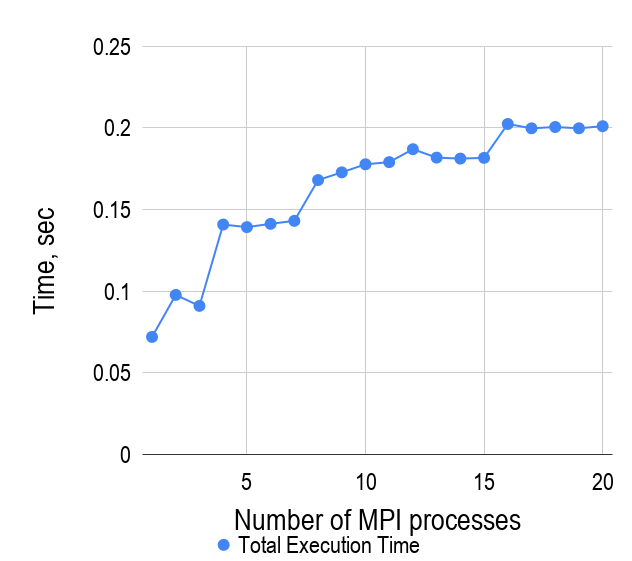
\includegraphics[width=0.475\textwidth]{figures/chapter-2/small-matrices/total-time-cube-5.png}} \\
	\end{tabular}
	\caption{MUMPS parallel performance in case of relatively small matrices}
	\label{fig:mumps-small-matrices-total-time}
\end{figure}


A simple profiling showed two important things. Firstly, numerical factorization time and time spent on the analysis phase had the same order in case of sequential execution i.e. 1 MPI process. Secondly, while numerical factorization time barely decreased with increase of number of processing units, time spent on analysis phase time significantly grew. The results of profiling are shown in figure \ref{fig:mumps-small-matrices-profiling}.\\


\figpointer{\ref{fig:mumps-small-matrices-profiling}}
\begin{figure}[htpb]
\centering
	\begin{tabular}{cc}
		\subfloat[pwr-3d]{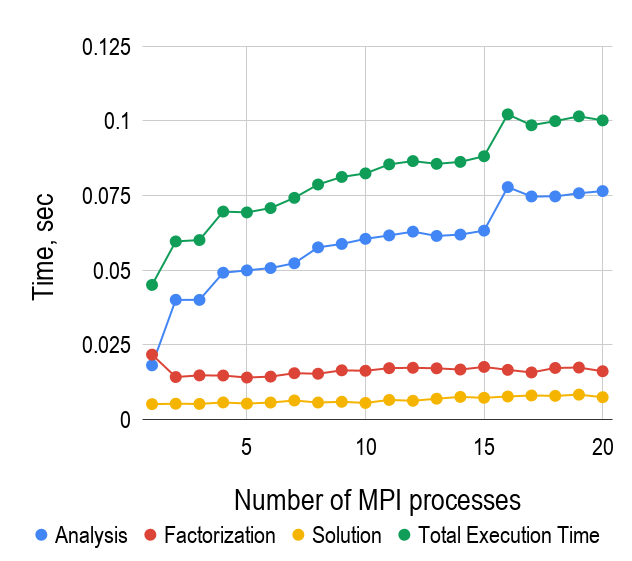
\includegraphics[width=0.475\textwidth]{figures/chapter-2/small-matrices/profiling-pwr-3d.png}} &
		\subfloat[cube-5]{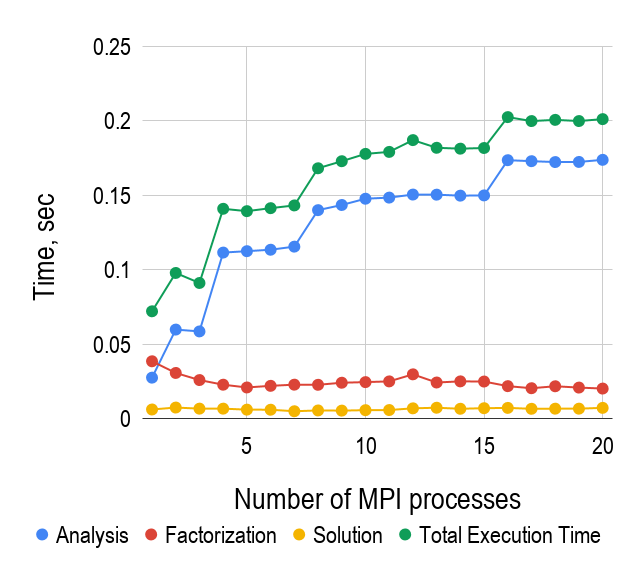
\includegraphics[width=0.475\textwidth]{figures/chapter-2/small-matrices/profiling-cube-5.png}} \\
	\end{tabular}
	\caption{Profiling of MUMPS library in case of factorization of relatively small matrices}
	\label{fig:mumps-small-matrices-profiling}
\end{figure}


It is obvious, according to the profiling results, the cause of such abnormal strong scaling behavior is  overheads induced by the analysis phase. A careful analysis of the graphs showed the analysis phase contained several peaks at points where the processor count was equal to a power of two. We assume that either fill reducing or process mapping pre-processing step can be a reason for that. However, in order to give the exact answer, detailed profiling and tracing of the analysis phase is required which is out of the scope of this study.\\


Interestingly, it turned out that even sequential execution of MUMPS for such small matrices was slower in contrast to a PETSc build-in sequential direct sparse solver. For example, in case of \textit{pwr-3d} matrix factorization, the PETSc build-in solver was almost 4 times faster than MUMPS. It is relevant to assume that PETSc solver does not have some additional overheads induced by adaptation of the solver for parallel execution. Hence, we can conclude that MUMPS is not the best choice for small matrices and thus we have to investigate another solvers available in PETSc for that range of systems.\\


As the first step, the following purely sequential solvers were compared with MUMPS for \textit{pwr-3d} and \textit{cube-5} test cases: KLU, PETSc built-in, SuperLU, UMFPACK. The results of the comparison are shown in figure \ref{fig:sequntial-solvers-comparison}.


\todo{TOTAL TIME}
\figpointer{\ref{fig:sequntial-solvers-comparison}}
\begin{figure}[htpb]
\centering
	\begin{tabular}{cc}
		\subfloat[pwr-3d]{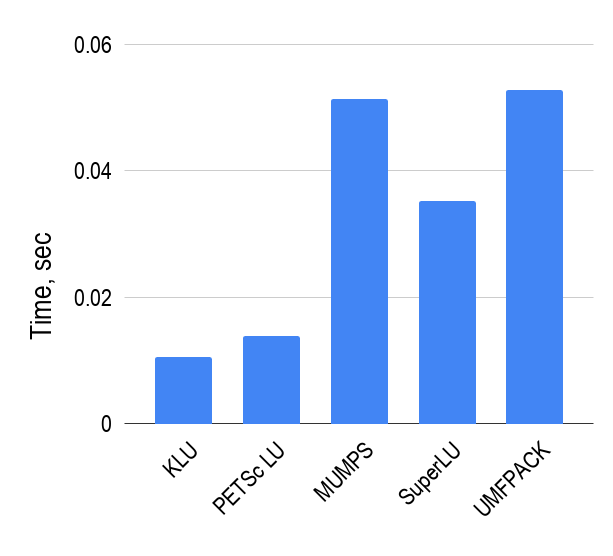
\includegraphics[width=0.475\textwidth]{figures/chapter-2/small-matrices/sequencial-solvers-comparison-pwr-3d.png}} &
		\subfloat[cube-5]{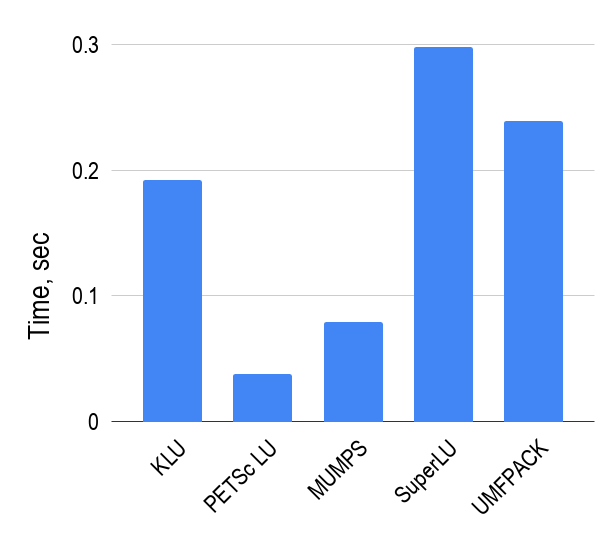
\includegraphics[width=0.475\textwidth]{figures/chapter-2/small-matrices/sequencial-solvers-comparison-cube-5.png}} \\
	\end{tabular}
	\caption{Comparison of sequential direct sparse solvers available in PETSc tested for relatively small matrices}
	\label{fig:sequntial-solvers-comparison}
\end{figure}


According the results, in general, the built-in PETSc solver performs better than the other tested solvers. We noticed that KLU was the fastest only in case of \textit{pwr-3d} matrix. But, at the same time, its performance drops significantly for the second test case and it becomes almost 4 times slower than PETSc solver. It is interesting to notice that performance of MUMPS considerably improves between two tests relatively to the PETSc solver. While it is approximately BRA times slower in case of \textit{pwr-3d} matrix factorization, it becomes only BRA-BRA slower for \textit{cube-5} test scenario. Taking all results and data into consideration, we chose PETSc implementation as the main sequential solver for small systems of equations for our following study.\\



We assume there exist a point i.e. the number of equations in a system, where MUMPS performance reaches the same level as the built-in PETSc solver. It is legitimate to think that analysis phase overheads become negligible after the point and MUMPS begins to work efficiently in parallel. Obviously, the point can vary form system to system and probably depends on the matrix sparsity pattern, the number of equation in a system and underlying PDE discretization. These make it impossible to predict the point exactly for a general matrix. However, it may be possible to make a general guidance for matrices generated by ATHLET (GRS software) since all matrices usually come from the same PDE discretization and are about in the same matrix density rage i.e. $nnz / n = {6 \dots 14}$. In order to develop such a guidance, an additional test was designed to find an approximate point for switching.\\


An application was developed to generate a Poisson matrix, based on 7-point stencil, with variable size for the test. During the test, we gradually increased the size and measured performance of both MUMPS and PETSc running sequentially as the direct solvers. The test results are represented in figure BRA.\\


% 5. Show the point where we have to switch to MUMPS in case of 7-point stencil

\todo{show the intersection point}
\todo{ZOOMING}

% Generate two other matrices with CUBE scenario and show that it works.

% conclusions

